\begin{Problem}
	In einem Wassertank befinden sich 10 Liter Wasser, mit einem Zulauf- und Ablaufrohr. Durch das Zulaufrohr kommt Wasser mit 2 Liter pro Minute in den Wassertank. Beim Ablaufrohr fließt die gleiche Menge ab. Weiterhin zirkuliert das Wasser im Wassertank permanent.

Zur Zeit \(t_0 = 0\) ist nur reines Wasser im Wassertank. Nun wird ab \(t_0 = 0\) bei dem Zulaufrohr Salz mit \(0{,}3\) Kilogramm pro Liter hinzugefügt (das Salz ist bereits im Wasser gelöst). Im Wassertank vermischen sich durch die Zirkulation Wasser und Salz gleichmäßig, das heißt wir gehen immer davon aus, dass das Salz im Wassertank gleichmäßig verteilt ist. Im Folgenden sei \(x(t)\) der Salzgehalt (in Kilogramm) im Wassertank zum Zeitpunkt \(t\) (in Minuten).

\begin{center}
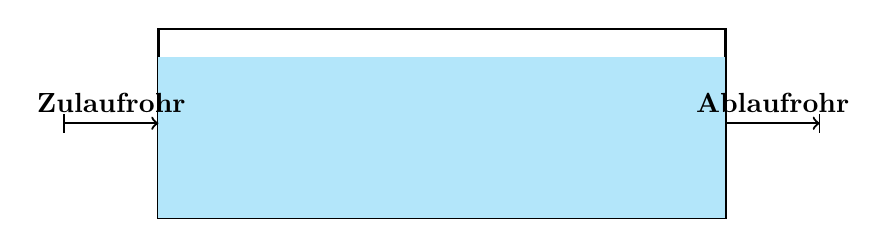
\begin{tikzpicture}[scale=1.2]
    % Tank
    \draw[thick] (0,0) rectangle (6,2);
    \fill[cyan!30] (0,0) rectangle (6,1.7);
    % Zulaufrohr
    \draw[thick,->] (-1,1) -- (0,1) node[midway,above]{\textbf{Zulaufrohr}};
    \draw (-1,0.9) -- (-1,1.1);
    % Ablaufrohr
    \draw[thick,->] (6,1) -- (7,1) node[midway,above]{\textbf{Ablaufrohr}};
    \draw (7,0.9) -- (7,1.1);
\end{tikzpicture}
\end{center}

\textbf{Abbildung 1:} Wassertank mit Zulauf- und Ablaufrohr

\begin{enumerate}
    \item[(a)] Leiten Sie die Differentialgleichung \(\dot{x} = f(x)\) her, die die Änderung des Salzgehalts im Wassertank beschreibt.
    \item[(b)] Bestimmen Sie eine Formel zur Berechnung des Salzgehalts \(x(t)\) im Wassertank.
    \item[(c)] Geben Sie den Salzgehalt im Wassertank nach 5 Minuten an.
    \item[(d)] Bestimmen Sie den Salzgehalt im Wassertank, der sich auf lange Zeit einstellen würde.
\end{enumerate}
\end{Problem}
\begin{proof}
	\begin{parts}
	\item Sei $x$ das Salzgehalt im Wassertank. In einem kleinen Zeitintervall $\dd{t}$ kann man sich vorstellen, dass $2 / 10 \cdot x\dd{t}$ Salz das Wassertank verlässt, da das Salz gleichmäßig verteilt ist.

		Gleichzeitig wird $(2\dd{t})\cdot 0.3$ Salz durch das Zulaufrohr reingebracht. Damit ist
		\[
			\dd{x} = 0.6 \dd{t} - 0.2 x\dd{t}
		\]
		oder
		\[
			\dot{x} = 0.6 - 0.2x
		.\] 
	\item Der Anfangswert ist $x = 0$. Wir l\"{o}sen die DGL durch TDV
		\[
			\int_0^x \frac{1}{0.6-0.2s}\dd{s} = \int_0^t \dd{t}
		\]
		mit L\"{o}sung
		\[
			x=3(1-e^{-0.2t})
		.\] 
	\item $1.90$ kg/L.
	\item $\displaystyle \lim_{t \to \infty} x(t) = 3$ kg/L.
	\end{parts}
\end{proof}
\begin{Problem}
	Es sei $\varphi : I \to \R^2$ eine von Null verschiedene Lösung von
	\begin{align*}
		\dot{x}_1&=-x_1+x_2-x_1^3\\
		\dot{x}_2&=-x_1-x_2-x_2^3
	\end{align*}
	\begin{parts}
	\item Zeigen Sie, dass die Funktion $I\to \R,~t\mapsto \|\varphi(t)\|$ nie $0$ werden kann und streng monoton fallend ist.
	\item Zeigen Sie, dass $I$ nach rechts unbeschränkt ist und $\lim_{t\to\infty} \varphi(t)=0$.
	\end{parts}
\end{Problem}
\begin{proof}
	\begin{parts}
	\item $\|\varphi(t)\|=0$ nur wenn $x_1=x_2=0$. Aber man sieht, dass $x_1(t)=x_2(t)=0$ eine L\"{o}sung der DGL mit Anfangswert $(0,0)$ ist. Weil die rechte Seite nach $x_1$ und $x_2$ stetig differenzierbar ist, ist sie lokal lipschit Stetig und die L\"{o}sung ist lokal eindeutig, was ein Widerspruch wäre, wenn $\|\varphi(t)\|$ 0 wird.

		Wir betrachten $\|\varphi(t)\|^2$. Es gilt
		\begin{align*}
			\dv{t}\|\varphi(t)\|^2 &= 2x_1\dot{x}_1 + 2x_2\dot{x}_2\\
					       &=2x_1(-x_1+x_2-x_1^3) + 2x_2(-x_1-x_2-x_2^3)\\
					       &=-2(x_1^2+x_1^4+x_2^2+x_2^4)\\
					       &< 0
		\end{align*}
		(strikt kleiner als 0, weil $\|\varphi(t)\|\neq 0$.)
	\item Sei $\|\varphi(0)\|=R$. Dann ist $\phi(t) \in \overline{B_r(0)}$ f\"{u}r all $t\in I$. Wenn $I$ nach rechts beschränkt wäre
	\end{parts}
\end{proof}
